% =====================================================================
%  Chapter 2 --- Business Understanding, Requirements & Architecture
% =====================================================================
\chapter{Business Understanding, Requirements and Architecture}
\label{chap:business}

\section{Introduction}
Building on the strategic outline of Chapter~\ref{chap:context}, the present chapter formalizes the first phase of the CRISP-DM methodology: the \emph{business understanding}. The chapter restates the business objectives of the project in operational terms, formulates the research questions that drive the analytical work, derives the functional and non-functional requirements of the platform, presents the target software architecture --- with explicit attention to the MySQL-to-PostgreSQL bridge and to the secure remote-collaboration setup mandated by the binomial organization --- and concludes by justifying the technology stack adopted for the implementation.

\section{Business objectives}

\subsection{Strategic objectives of the host organization}
At the strategic level, three priorities of \hostorg{} converge towards the present project. The first is the \emph{operational risk reduction} of the customer fleets, by surfacing devices and vehicles whose behavioural pattern significantly deviates from the fleet baseline; this priority directly motivates the introduction of a continuous risk score on top of the existing descriptive reports. The second is the \emph{differentiation of the SaaS offering} through the addition of an advanced analytical layer that complements the dashboards already exposed to the customers. The third is the \emph{architectural decoupling} between the operational MySQL databases and the analytical workloads, in order to avoid contention with the live customer-facing traffic; this priority motivates the constitution of a dedicated analytical PostgreSQL warehouse, hosted in a controlled cloud environment.

\subsection{From observation to anticipation}
The existing analytical surface of \hostorg{} answers retrospective questions: \emph{what happened on the fleet last month?} \emph{how many overspeed events were recorded?} \emph{what was the total mileage per vehicle?} The project deliberately moves the analytical centre of gravity from observation to anticipation by introducing three additional capabilities: a behavioural \emph{segmentation} that groups devices into operational profiles, an \emph{anomaly score} that ranks devices by deviation from the tenant baseline, and a \emph{risk band} that translates the score into an operational priority for the fleet manager. These capabilities turn the platform into a decision-support layer rather than a passive observation layer.

\subsection{Operational objectives of the project}
The strategic priorities decompose into five concrete operational objectives:

\begin{enumerate}
    \item repatriate the relevant slices of the three operational MySQL databases of \hostorg{} into a dedicated analytical environment, through a reproducible MySQL-to-PostgreSQL conversion bridge;
    \item replace any ad-hoc, full-refresh analytical recomputation by an incremental, watermark-driven architecture with sub-ten-minute freshness;
    \item materialize a clean dimensional warehouse and a family of marts dedicated respectively to machine learning and to business intelligence;
    \item train an unsupervised behavioural segmentation and a continuous risk score per device-month, exposed through an API and a BI dashboard;
    \item industrialize the pipeline on the Azure VM through Prefect orchestration, cron scheduling and an explicit monitoring layer, while granting the binomial of students secure remote access.
\end{enumerate}

\section{Research questions}
Three research questions structure the analytical investigation:

\begin{enumerate}
    \item[\textbf{RQ1}] \emph{Can the heterogeneous behavioural signals of a multi-tenant telematics fleet --- recorded as raw hexadecimal telemetry, decoded \texttt{arch\_xxxxx} archive rows and \texttt{user\_xxxxx} master data --- be condensed into a small set of interpretable indicators at the device-month grain, without losing operational meaning?}
    \item[\textbf{RQ2}] \emph{Can these indicators be exploited by an unsupervised model in order to produce an actionable behavioural segmentation and a continuous risk score, in the absence of a labelled incident feed?}
    \item[\textbf{RQ3}] \emph{Can the resulting analytical outputs be served to fleet managers through a low-latency API and an interactive dashboard, hosted on a shared Azure infrastructure, without compromising the idempotency, the observability and the cost profile of the production pipeline?}
\end{enumerate}

\section{Requirements analysis}

\subsection{Functional requirements}
The functional requirements of the platform are summarized in Table~\ref{tab:fr}. Each requirement is identified by a code (\texttt{FR-x}), a short description and a priority level on a three-tier scale (high, medium, low).

\begin{table}[h]
\centering
\caption{Functional requirements.}
\label{tab:fr}
\begin{tabular}{|l|p{8.6cm}|c|}
\hline
\textbf{ID} & \textbf{Description} & \textbf{Priority} \\
\hline
FR-1 & Convert MySQL dump files (\texttt{arch\_xxxxx}, \texttt{user\_xxxxx}) into a PostgreSQL-importable representation. & High \\
FR-2 & Ingest the converted data into the analytical staging schema. & High \\
FR-3 & Apply the eleven cleaning rules and quarantine rejected rows. & High \\
FR-4 & Materialize five dimensions and eleven facts with idempotent upserts. & High \\
FR-5 & Build the device-month behavioural mart and the telemetry mart. & High \\
FR-6 & Train the per-tenant K-Means and Isolation Forest models. & High \\
FR-7 & Expose the cluster assignments and risk scores through a REST API. & High \\
FR-8 & Provide an interactive BI dashboard for fleet managers. & High \\
FR-9 & Run the pipeline incrementally every five minutes via cron. & High \\
FR-10 & Persist a run log and a data-quality measurement at every cycle. & Medium \\
FR-11 & Support full backfill and bootstrap modes for historical loads. & Medium \\
FR-12 & Support secure remote operations via SSH tunnelling and IP allowlist for the binomial. & High \\
FR-13 & Document the feature registry and the validation suite. & Medium \\
\hline
\end{tabular}
\end{table}

\subsection{Non-functional requirements}
The non-functional requirements are summarized in Table~\ref{tab:nfr}.

\begin{table}[h]
\centering
\caption{Non-functional requirements.}
\label{tab:nfr}
\begin{tabular}{|l|p{8.6cm}|c|}
\hline
\textbf{ID} & \textbf{Description} & \textbf{Target} \\
\hline
NFR-1 & End-to-end pipeline latency. & $\le 10$ minutes \\
NFR-2 & Idempotency on full re-runs. & 100\% \\
NFR-3 & Pipeline availability on the Azure VM. & $\ge 99\%$ \\
NFR-4 & Mean cycle time for incremental mode. & $\le 60$ seconds \\
NFR-5 & Coverage of the validation suite (V1--V8). & 100\% per run \\
NFR-6 & Secure access (SSH key + IP allowlist). & Mandatory \\
NFR-7 & Reproducibility (random seed, pinned versions). & Mandatory \\
NFR-8 & Per-tenant fairness of the model quality. & Silhouette $\ge 0.15$ \\
NFR-9 & Isolation from the operational MySQL workload. & No reads on production peak hours \\
\hline
\end{tabular}
\end{table}

\subsection{User profiles}
Three user profiles consume the outputs of the platform:

\begin{itemize}
    \item \emph{Fleet managers} consult the BI dashboard, filter by tenant and device, and act on the risk score and on the cluster assignments.
    \item \emph{Data engineers} maintain the pipeline, monitor the run log, replay backfills and adjust the cleaning rules and the feature registry.
    \item \emph{Data scientists} consume the ML view, retrain the models on extended windows and propose iterations of the feature set.
\end{itemize}

\section{Target architecture}

\subsection{Logical view}
At the logical level, the platform is organized as a four-tier architecture that explicitly mirrors the lifecycle of a telemetry signal: a \emph{source tier} represented by the three operational MySQL databases of \hostorg{} (raw hex telemetry, decoded \texttt{arch\_xxxxx} archive, \texttt{user\_xxxxx} master data); a \emph{conversion and ingestion tier} that exports MySQL dumps, converts them to PostgreSQL-compatible files and loads them into staging; a \emph{processing and storage tier} composed of the staging, warehouse and marts schemas of the analytical PostgreSQL, transformed by Python and SQL tasks orchestrated by Prefect; and a \emph{serving tier} composed of the API, the BI dashboard and the model artefact store.

\subsection{Physical view on Microsoft Azure}
At the physical level, the platform is hosted on a Microsoft Azure virtual machine running a recent Linux distribution. The analytical PostgreSQL instance, the Python virtual environment, the Prefect flow, the cron entry, the API and the dashboard are co-located on this VM. Two binomial members access the VM through SSH key authentication; an explicit IP allowlist enforced by an Azure Network Security Group attached to the VM restricts inbound SSH connections to the two students' workstations and to the office network of \hostorg. Database access from local notebooks of the binomial passes through an SSH tunnel terminating on \texttt{localhost:5432} of the VM, so that the PostgreSQL port is never exposed to the public internet.

\subsection{Data flow}
The data flow is represented in Figure~\ref{fig:dataflow}. MySQL dump files are exported from the operational system of \hostorg, converted to PostgreSQL by dedicated scripts, loaded into the staging schema, processed by the cleaning engine into the warehouse layer, condensed into the marts and finally consumed either by the API and the dashboard or by the offline modeling notebooks.

\begin{figure}[h]
\centering
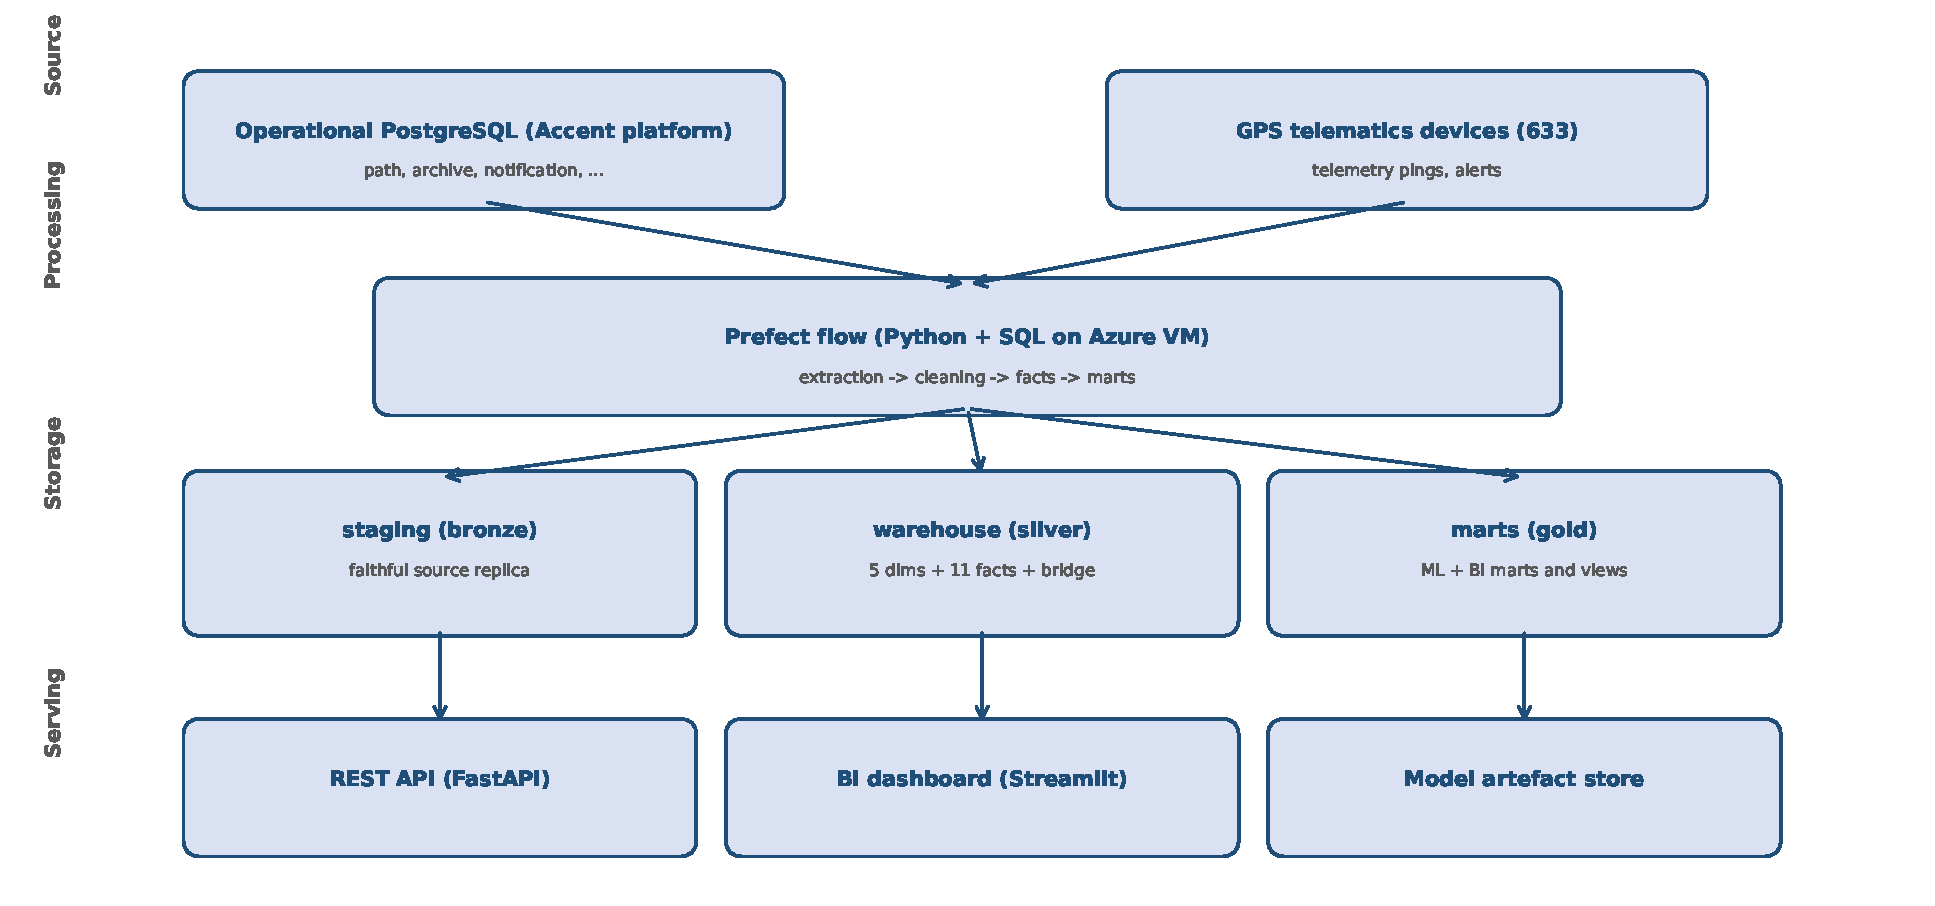
\includegraphics[width=0.95\textwidth]{figures/architecture_dataflow.pdf}
\caption{Logical data flow of the platform, from MySQL sources to PostgreSQL marts.}
\label{fig:dataflow}
\end{figure}

\subsection{Layered storage}
The storage tier is organized as a three-layer warehouse: the \emph{bronze} layer (\texttt{staging}) hosts a faithful PostgreSQL replica of the converted MySQL data, the \emph{silver} layer (\texttt{warehouse}) hosts the dimensional model with deduplicated facts and dimensions, and the \emph{gold} layer (\texttt{marts}) hosts the business-ready aggregates. State tables (\texttt{etl\_watermark}, \texttt{etl\_run\_log}, \texttt{quarantine\_rejected}) live alongside the warehouse layer and support the operational concerns of the pipeline.

\section{Technology stack}

\subsection{Operational source: MySQL}
The operational source of the project is the MySQL stack of \hostorg, which carries the three databases described in Chapter~\ref{chap:context}. The project does not modify these databases in any way; it consumes them through periodic dump files (\texttt{.sql}) provided by the engineering team of \hostorg. The dumps cover the slices of the \texttt{arch\_xxxxx} archive and the \texttt{user\_xxxxx} master data that are required for the analytical scope.

\subsection{Analytical warehouse: PostgreSQL~16}
The analytical warehouse is implemented in PostgreSQL~16, chosen for its strong support of analytical workloads, its ACID guarantees, its advanced indexing, its scalability to large datasets, its extensibility and its first-class compatibility with the Python data ecosystem and with standard BI tools. The detailed justification of this choice is given in \S\ref{ssec:why-postgres}. PostgreSQL is hosted on the Azure VM, with public ports closed and access mediated by SSH tunnelling.

\subsection{Why PostgreSQL rather than MySQL for the warehouse}
\label{ssec:why-postgres}
The decision to host the analytical layer on PostgreSQL rather than on the same MySQL stack as the operational system rests on six independent technical criteria:

\begin{enumerate}
    \item \textbf{Analytical SQL surface.} PostgreSQL exposes a rich set of analytical idioms --- window functions over arbitrary partitions, common table expressions (recursive included), \texttt{LATERAL} joins, set-returning functions, \texttt{FILTER} clauses on aggregates --- that condense behavioural feature definitions into compact, readable SQL. The same logic in operational MySQL would require lengthier and more error-prone query rewrites.
    \item \textbf{ACID compliance and crash safety.} The full ACID semantics of PostgreSQL on \texttt{INSERT~\dots~ON~CONFLICT~DO~UPDATE} and on transactional DDL are required by an unattended pipeline that runs every five minutes and must survive partial failures without manual intervention.
    \item \textbf{Advanced indexing.} The native availability of B-tree, BRIN, GIN, partial and expression indexes covers the access patterns of the analytical layer (range scans on time, aggregate filters, JSON inspection) much more naturally than the indexing options of the operational MySQL setup.
    \item \textbf{Scalability to large datasets.} PostgreSQL handles the volumes considered by the project --- of the order of \(10^7\) telemetry rows --- without the architectural retrofitting that the same volume would require on a MySQL warehouse retrofitted from an operational instance.
    \item \textbf{Extensibility.} The PostgreSQL extension ecosystem (\texttt{pg\_stat\_statements} for workload telemetry, \texttt{postgis} for geospatial enrichment, \texttt{pg\_partman} for partitioned tables) opens forward trajectories that fit the analytical roadmap of \hostorg{}.
    \item \textbf{Compatibility with data warehousing and BI tools.} The PostgreSQL JDBC and \texttt{psycopg2} drivers, the wide adoption by orchestration frameworks (Prefect, Airflow), by Python (pandas, SQLAlchemy) and by BI clients (Streamlit, Plotly Dash, Metabase, Power BI through ODBC) make PostgreSQL the path of least friction for the consumers of the warehouse.
\end{enumerate}

These criteria, together with the strategic decision of decoupling the analytical workload from the operational MySQL stack, justify the adoption of PostgreSQL as the analytical DBMS of the project.

\subsection{Conversion bridge: MySQL dumps to PostgreSQL}
A dedicated conversion bridge transforms the MySQL dump files received from \hostorg{} into PostgreSQL-importable artefacts. The bridge handles the dialect differences (data types, quoting conventions, default expressions, \texttt{AUTO\_INCREMENT} translation, character-set normalization) and produces \texttt{COPY}-friendly CSV or SQL files loaded into the staging schema. The detailed description of the bridge is given in Chapter~\ref{chap:prep}; at this stage it suffices to note that the bridge is part of the technology stack of the platform and that its outputs constitute the input of the staging layer.

\subsection{Processing and orchestration}
The processing layer is written in Python~3.11. Database access is implemented through SQLAlchemy and \texttt{psycopg2}; analytical transformations rely on \texttt{pandas} and \texttt{numpy}; the modeling layer relies on \texttt{scikit-learn}; the orchestration uses Prefect~2 to chain the tasks of the batch flow. A test suite is implemented with \texttt{pytest}.

\subsection{Modeling and machine learning}
The unsupervised modeling layer relies on \texttt{scikit-learn} (StandardScaler, KMeans, IsolationForest), with seed control and per-tenant fitting. A deep-learning baseline (PyTorch autoencoder) has been examined for comparison purposes (cf.\ Chapter~\ref{chap:model}).

\subsection{Serving, API and dashboard}
The API is implemented with FastAPI, exposed through Uvicorn behind an Nginx reverse proxy. The dashboard is implemented with Streamlit (or, equivalently, Plotly Dash), embedded on the same VM and connected to the marts schema. Both components are deployed as systemd services.

\subsection{Cloud and shared collaboration environment}
The cloud platform is Microsoft Azure. The VM is provisioned with a Linux image, a managed disk, an attached Network Security Group with an IP allowlist for SSH, and a static public IP. The git repository of the project is cloned into \texttt{/opt/accent-fleet-analytics}, the Python virtual environment is provisioned locally, and the cron entry under \texttt{/etc/cron.d/} triggers the incremental runs. The system journal collects the structured logs. The Azure VM constitutes the shared workspace of the binomial: both students connect to the same database and operate the same pipeline through their personal SSH keys, while the IP allowlist on the Network Security Group prevents any non-authorized host from reaching the VM.

\subsection{Justification of the technology choices}
The technology choices are justified by four criteria. \emph{Alignment} with the operational stack of \hostorg{} is preserved on the source side (MySQL is consumed without modification). \emph{Separation of concerns} is respected on the analytical side (PostgreSQL is dedicated to analytics). \emph{Maturity} of the Python data ecosystem (\texttt{scikit-learn}, \texttt{pandas}, Prefect) supports a binomial of student engineers without imposing rare or fragile components. \emph{Minimality} of the operational footprint --- every component runs on a single VM, with no managed Kubernetes cluster nor managed Spark cluster --- controls the cloud cost and keeps the surface of the system small enough to be operated by a binomial.

\section{Conclusion}
This chapter has formalized the business understanding of the project, derived the functional and non-functional requirements --- including the explicit MySQL-to-PostgreSQL conversion bridge and the requirements imposed by the binomial collaboration mode --- and presented the logical and physical architecture of the platform with a particular focus on the analytical PostgreSQL warehouse hosted on the Azure VM. The next chapter executes the data understanding phase by inspecting the three operational databases of \hostorg{} and by characterizing the slices that feed the analytical pipeline.
